% !TeX spellcheck = id_ID
\documentclass[a4paper,12pt]{article}
\usepackage[indonesian]{babel}
\usepackage{graphicx}
\usepackage{multirow}
\usepackage{enumitem}
\usepackage{listings}
\usepackage{wrapfig}
\usepackage[T1]{fontenc}
\usepackage{inconsolata}
\usepackage{lipsum}
\usepackage{adjustbox}


\usepackage{color}
\usepackage[table]{xcolor}
\definecolor{pblue}{rgb}{0.13,0.13,1}
\definecolor{pgreen}{rgb}{0,0.5,0}
\definecolor{pred}{rgb}{0.9,0,0}
\definecolor{pgrey}{rgb}{0.46,0.45,0.48}
%\lstset{language=Java,
%	showspaces=false,
%	showtabs=false,
%	breaklines=true,
%	showstringspaces=false,
%	breakatwhitespace=true,
%	commentstyle=\color{pgreen},
%	keywordstyle=\color{pblue},
%	stringstyle=\color{pred},
%	rulecolor=\color{black},
%	basicstyle=\ttfamily,
%	moredelim=[il][\textcolor{pgrey}]{$$},
%	moredelim=[is][\textcolor{pgrey}]{\%\%}{\%\%}
%}

\graphicspath{ {./img/} }
\begin{document}
\title{ {\Large Laporan Praktikum}\\ Algoritma dan Pemrograman \\{\Large Pertemuan 14}}

\author{Aldzikri Dwijayanto Prathama 
	\\195410189
	\\Teknik Informatika}
\makeatletter
\begin{titlepage}
	\begin{center}
		{\huge \bfseries \@title }\\[14ex]
		
\includegraphics[scale=.8]{logo}\\[4ex]
		{\large \@author}\\[19ex]
		{\large \bfseries {SEKOLAH TINGGI MANAJEMEN INFORMATIKA DAN KOMPUTER
				AKAKOM YOGYAKARTA}}
	\end{center}


%{\large \@date} 
\end{titlepage}
\makeatother
%\maketitle
\newpage
\tableofcontents
\newpage

\section{Tujuan}
\begin{enumerate}
    \item Mahasiswa dapat mengimplementasikan konsep Sekuensi, seleksi dan iterasi untuk menyelesaikan kasus yang sederhana
    \item Mahasiswa dapat mengubah dari satu bentuk seleksi ke bentuk seleksi yang lain begitu juga dalam perulangan
\end{enumerate}

\section{Dasar Teori}
Teori mengenai sekuensi, seleksi dan iterasi dapat dilihat pada modul pertemuan sebelumnya.

\newpage

\section{Praktik}
\subsection{Praktik 1}
Suatu rangkaian yang tersusun atas 3 resistor yang di pararel, buatlah diagram alir/flowchart yang meminta nilai R1, R2, R3 dari keyboard untuk menampilkan nilai
R dengan rumus :\\
R = 1/(1/R1+1/R2+1/R3)
\paragraph{Jawab}
\begin{center}
    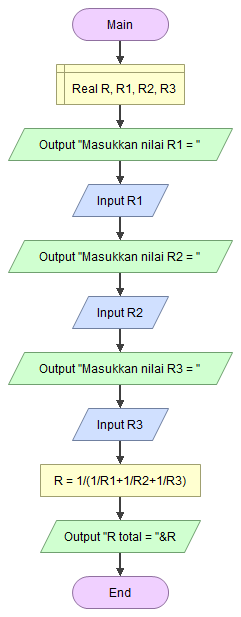
\includegraphics[height=.6\textheight]{praktik1 - Main.png}
\end{center}

\end{document}
